\documentclass[11pt,a4paper]{article}

\usepackage[english]{babel}
\usepackage[T1]{fontenc}
%\usepackage[latin1]{inputenc}

\usepackage{amsmath}
\usepackage{multirow}
%\usepackage[margin=2cm]{geometry}
\usepackage[dvipsnames]{xcolor}

\usepackage{graphicx}
\usepackage{amssymb}
\usepackage{mathrsfs}
\usepackage{subcaption}
\usepackage{setspace} 

\definecolor{AB}{rgb}{0,0.3961,0.7412}

\usepackage[bookmarksnumbered=true]{hyperref} 
\hypersetup{
     colorlinks = true,
     linkcolor = AB,
     anchorcolor = AB,
     citecolor = AB,
     filecolor = AB,
     urlcolor = AB
 }
\usepackage{enumitem}
\allowdisplaybreaks

\addtolength{\oddsidemargin}{-.8in}
\addtolength{\evensidemargin}{-.65in}
\addtolength{\textwidth}{1.68in}
\addtolength{\topmargin}{-.875in}
\addtolength{\textheight}{1.15in}

\usepackage{titlesec}
\titleformat{\section}{\fontsize{12}{14}\sc}{\thesection}{1em}{}[]
\titleformat{\subsection}{\fontsize{11}{12}\sc}{\thesubsection}{1em}{}[]
\titleformat{\subsubsection}{\fontsize{10}{11}\sc}{\thesubsection}{1em}{}[]
 
 \setlength{\parindent}{0pt}
 
\usepackage{tocloft}
\renewcommand{\cfttoctitlefont}{\sc}
\renewcommand{\cftsecfont}{\sc}
\renewcommand{\cftsubsecfont}{\sc}

\usepackage{abstract}
\renewcommand\abstractnamefont{\sc}

\usepackage[round]{natbib}

 
\begin{document}
\thispagestyle{empty}

\begin{flushleft} 
\includegraphics[width=1.0\textwidth]{headers}   \end{flushleft}

\vskip0.5cm
\begin{spacing}{2} {\Large\sc\noindent Optimum power for a set of $m$ lamps illuminating a set of $n$ flat patches to best approach a target illumination}
\end{spacing}

\vfill

\begin{spacing}{1.2}
{\large\sc  Antonio Felype Ferreira Maciel - 576261}\\

{\noindent \large \sc Master's Course in Teleinformatics Engineering}\\
{\noindent \large \sc Federal University of Ceará}\\

{\noindent \large \sc TIP8300 - Nonlinear System Optimization}
\end{spacing}

\newpage 

\tableofcontents

\newpage

%\begin{abstract}
% This report provides a concise introduction to Up-flow Anaerobic Sludge Blanket reactor, outlines its applications in Brazil, and explains the model we are using for simulations. We discuss our intentions for using this model, the challenges we are currently facing and our next steps. 
%\end{abstract}

\section{Problem Definition}

Consider $m$ lamps illuminating $n$ (small flat) patches. The illumination intensity $I_k$ at the $k$-th patch depends linearly on the lamp power $p_j$ as:
\begin{equation*}
    I_k = \displaystyle \sum_{j=1}^{m}a_{k,j}p_j, \quad \text{with} \, a_{k,j} = r_{k,j}^{-2}\max\{\cos(\theta_{k,j}),0\},
\end{equation*}

where $r_{k,j}$ is the length of the vector $r_{k,j}$ connecting the center of the $k$-th patch to the position of the $m$-th lamp and $\theta_{k,j}$ is the angle between the patch normal vector $\mathbf{n}_k$ and $\mathbf{r}_{k,j}$. See the Convex Optimization book slides for more details.\\

The proposed problem is to achieve a desired illumination $I_{des}$ with bounded lamp powers ($p_{max}$), i.e.,
\begin{align*}
    \min & \quad \underset{k=1,2,\dots,n}{\max}\vert \log{(I_k)} - \log{(I_{des})} \vert \\
    \text{s.t.} & \quad 0 \leq p_j \leq p_{max}, j = 1, 2, \dots, m.
\end{align*}

\begin{itemize}
    \item[] Suboptimally solve the problem using, e.g., Python or Octave, according to the following approaches:
    \item[] \begin{enumerate}
        \item Using uniform power, i.e., $p_j = p, 0 \leq p \leq p_{max}$.
        \item Using least-squares, i.e., $\min . \displaystyle \sum_{k=1}^{n} (I_k - I_{des})^2$, and rounding $p_j$ as $p_j = \max\{0, \min\{p_j, p_{max}\}\}$.
        \item Using weighted least-squares, i.e., $\min . \displaystyle \sum_{k=1}^{n}(I_k - I_{des})^2 + w_j\sum_{j=1}^n (p_j - p_{max})^2$ and iteratively adjusting the weights $w_j$ until $0 \leq p \leq p_{max}, \forall j$.
        \item Using linear programming, i.e., 
        \begin{align*}
            \min & \quad \underset{k=1, 2, \dots, n}{\max} \vert I_{k} - I_{des} \vert \\
            \text{s.t.} & \quad 0 \leq p_j \leq p_{max}, \quad j = 1, 2, \dots, m.
        \end{align*}
    \end{enumerate}
    \item[] Solve the problem optimally using convex optimization.
        
        For this goal, consider the equivalent convex problem
        \begin{align*}
            \min & \quad \underset{k = 1, 2, \dots, n}{\max} h\left(\cfrac{I_k}{I_{des}}\right) \\
            \text{s.t.} & \quad 0 \leq p_j \leq p_{max}, \quad j = 1, 2, \dots, m, 
        \end{align*}
    
        where $h(u) = \max\left\{u, \cfrac{1}{u}\right\}$.
\end{itemize}

For this work, $n = 4$ lamps illuminating $m = 5$ patches are considered. Matrices $P_l$ and $P_{p}$ contain the $x$ and $y$ coordinates of the lamps and the patches' ends, respectively (\ref{eq:positions}). Figure~\ref{fig:lamps-patches-position} shows how the lamps and the patches are displayed. 

\begin{equation*}
    P_l = \begin{bmatrix}
        0.7609 & 6.9497\\
        1.9382 & 8.0610\\
        4.4674 & 6.7316\\
        7.4095 & 7.3987
    \end{bmatrix}
    \quad
    P_{p} = \begin{bmatrix}
        0.1329 & 3.9041\\
        1.5435 & 2.6782\\
        3.3102 & 3.3981\\
        4.7796 & 2.2716\\
        5.8071 & 2.4345\\
        7.0621 & 2.1015
    \end{bmatrix}
    \label{eq:positions}
\end{equation*}

\begin{figure}[!htb]
    \centering
    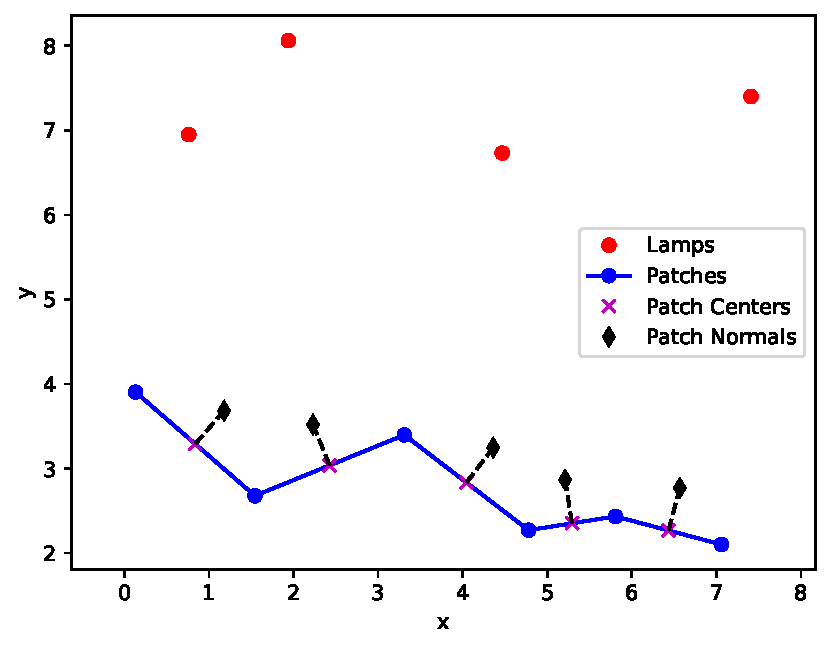
\includegraphics[width=0.5\textwidth]{figures/lamps-patches-position.pdf}
    \caption{Lamps and patches positions.}\label{fig:lamps-patches-position}
\end{figure}

\newpage

\section{Suboptimal approaches}

All the code developed for this work is avaiable online\footnote{\href{https://github.com/felypemaciel/lamps/blob/main/lamps.ipynb}{Lamps and Patches - GitHub Repository}}.

\subsection{Uniform power}

For this approach, a value of power $p$ is assumed to be the same for all the lamps. By varying the value of $p$, it is possible to see how the illuminations of each patch behave.\\

Figure~\ref{fig:uniform-power} shows how the illumination in each patch evolves as the power $p$ grows. We see that the desired illumination is met for each patch at different values of $p$. In this manner, even though it is possible to reach the desired illumination for a patch, the others either have less or more illumination that they should.\\

\begin{figure}[!htb]
    \centering
    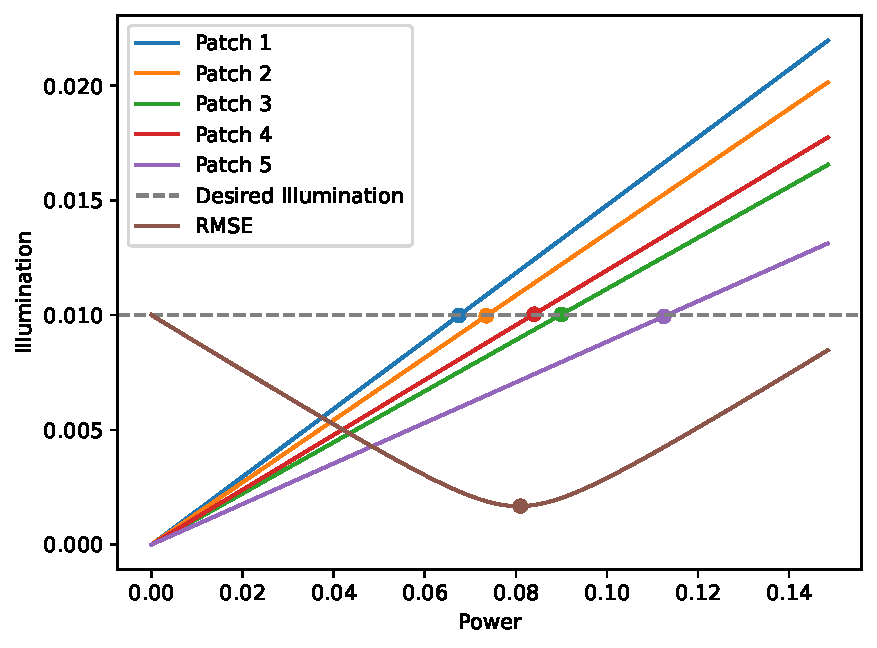
\includegraphics[width=0.55\textwidth]{figures/uniform-power.pdf}
    \caption{Patches' illumination when varying a uniform power.}\label{fig:uniform-power}
\end{figure}

The RMSE curve shows how the RMSE varies for the power variation. The power that minimizes it used to calculate the illumination coefficients, which are shown in Table~\ref{tab:uniform-power}.

\begin{table}[!htb]
    \centering
    \caption{Illumination results for uniform power.}
    \begin{tabular}{lccccc}
        \hline
        & Patch 1 & Patch 2 & Patch 3 & Patch 4 & Patch 5\\
        Illumination & 0.012 & 0.011& 0.009& 0.0097& 0.0072\\
        \hline
    \end{tabular}\label{tab:uniform-power}
\end{table}

\subsection{Least-squares}

In the least-squares approach, we aim at determining the vector of powers $p$ that minimizes the squared difference between the patche's illuminations and the desired illumination (\ref{eq:least-squares}).
\begin{equation}
    \min \displaystyle \sum_{k=1}^{n} (I_k - I_{des})^2
    \label{eq:least-squares}
\end{equation}

In this approach, it is not possible to set the constraints for $p$, i.e., ($0 <= p <= p_{max}$). A possible way to get over this is to set negative elements of $p$ to 0 and values greater than $p_{max}$ to be equal to $p_{max}$, i.e., $p_j = max\{0, min\{p_j, p_{max}\}\}$.\\


The matrix form of the problem is $\min (Ap - I_{des})^2,$, where $A$ is the matrix of illumination coefficients $a_{kj}$, that represent the illumination coefficient of lamp j to the patch k. $p$ is the vector of lamps powers. Each element of $Ap$ gives the illumination of a patch.\\

The least-squares problem has a closed form for determining $p$, which is $p = (A^T A)^{-1} A^T I_{des}$.\\

From Table~\ref{tab:least-squares} it is possible to see that the solution obtained through least-squares produces illuminations quite close the desired. However, since it does not have constraints, there are lamps with negative powers (Table \ref{tab:least-squares-power}). Additionally, the solution could also have lamps using more power than it was established. 
When fixing the negative powers, the patches' ilumination become far away from the desired.

\begin{table}[!htb]
    \centering
    \caption{Illumination results for least-squares.}
    \begin{tabular}{lccccc}
        \hline
        & Patch 1 & Patch 2 & Patch 3 & Patch 4 & Patch 5\\
        Not constrained & 0.0101 & 0.00982 & 0.00967 & 0.0105 & 0.00989\\
        Constrained & 0.0378 & 0.0369 & 0.0211 & 0.0255 & 0.0177\\
        \hline
    \end{tabular}\label{tab:least-squares}
\end{table}

\begin{table}[!htb]
    \centering
    \caption{Lamps power obtained with least-squares.}
    \begin{tabular}{lcccc}
        \hline
        & Lamp 1 & Lamp 2 & Lamp 3 & Lamp 4\\
        Power & -0.399 & 0.944 & -0.143 & 0.192\\
        \hline
    \end{tabular}\label{tab:least-squares-power}
\end{table}

\subsection{Weighted least-squares}

In the weighted least-squares approach, we aim at minimizing a function composed of the least-squares approach function and the squared difference between the vector $p$ and $p_{max}$, weighted by coefficients $w$. 
\begin{equation*}
    \min \displaystyle \sum_{k=1}^{n}(I_k - I_{des})^2 + w_j\sum_{j=1}^n (p_j - p_{max})^2
\end{equation*}

The purpose of this additional term is to penalise the cost function for values of $p_j$ that deviate from $p_{max}$. The coefficient $w_j$ determines how strong this penalty is, and it can be adjusted to meet the constraints for $p$: $0 \leq p \leq p_{max}$. In this approach, the weights must be iteratively be changed to meet the constraints.\\

This problem also has a closed form for $p$ (\ref{eq:p-weighted-least-squares}), where $W \in \mathbb{R}^{m \times m}$ is the diagonal matrix of weights.
\begin{equation}
    p = (A^T A + W)^{-1} \cdot (A^T I_{des} + W p_{max})
    \label{eq:p-weighted-least-squares}
\end{equation}

Using this approach, we aim at finding solutions that minimizing the squared error between the patch illumination and the desired illumination, while also minimizing the squared difference between the lamps powers and the maximum power. This tends to produce solutions that have values near to $p_{max}$. This would not be interesting if we would also like to minimize the total power used by the lamps.\\

Regarding to obtain solutions that respect the power constraints, the approach meets what is required. The patches also illuminations not too distance from the deisred. The final solution also depends on how the weights are iterated to meet the requirements.

\subsection{Linear programming}

In the linear programming approach, we aim at formulate the problem such that it has a linear objective function and linear constraints. The proposed problem is to minimize the maximum of the absolute difference between the illumination of a patch and the desired illumination. 

\begin{align*}
    \min & \quad \underset{k=1, 2, \dots, n}{\max} \vert I_{k} - I_{des} \vert \\
    \text{s.t.} & \quad 0 \leq p_j \leq p_{max}, \quad j = 1, 2, \dots, m.
\end{align*}

We can introduce a new variable $t$, such that $t \leq |I_k - I_{des}|, \quad \forall k = 1, \dots, n $. However, the absolute value is a nonlinear function. 

This way, we can add linear inequalities to contour this problem, such as
\begin{align*}
    t \geq & I_k - I_{des}, \quad \forall k\\
    t \geq & -(I_k - I_{des}) \quad \forall k.
\end{align*}

The linear programming problem can then be defined as
\begin{align*}
    \min \quad & t\\
    s.t. \quad & t \geq I_k - I_{des} \\
               & t \geq -(I_k - I_{des}) \\
               & 0 \leq p_j \leq p_{max}, \quad j = 1, \dots, m
\end{align*}

The Linear Programming approach produces illuminations quite close to the desired without consuming much power as the previous approach. 

\section{Optimal approach: Convex optimization}

In this approach, the problem is formulated as to minimize an equivalent convex function 
\begin{align*}
    \min \quad &  \underset{k = 1, 2, \dots, n}{\max} h\left(\cfrac{I_k}{I_{des}}\right) \\
    \text{s.t.} \quad & 0 \leq p_j \leq p_{max}, \quad j = 1, 2, \dots, m,
\end{align*}

where $h(u) = \max\left\{u, \cfrac{1}{u}\right\}$.

As $I_k$ approaches $I_{des}$, the fraction $\cfrac{I_k}{I_{des}}$ gets closer to 1. The function $h(I_k/I_{des})$ produces great values when $I_k < I_{des}$ and linearly crescent values when $I_k > I_{des}$. This way, $h(\cdot)$ has as its minimum the value 1, i.e., when $I_k = I_{des}$. This way, when minimizing $h(\cdot)$, we are aiming at minimizing the difference between $I_k$ and $I_{des}$. Figure~\ref{fig:convex-function} shows the behaviour of $h(\cdot)$.

\begin{figure}[!htb]
    \centering
    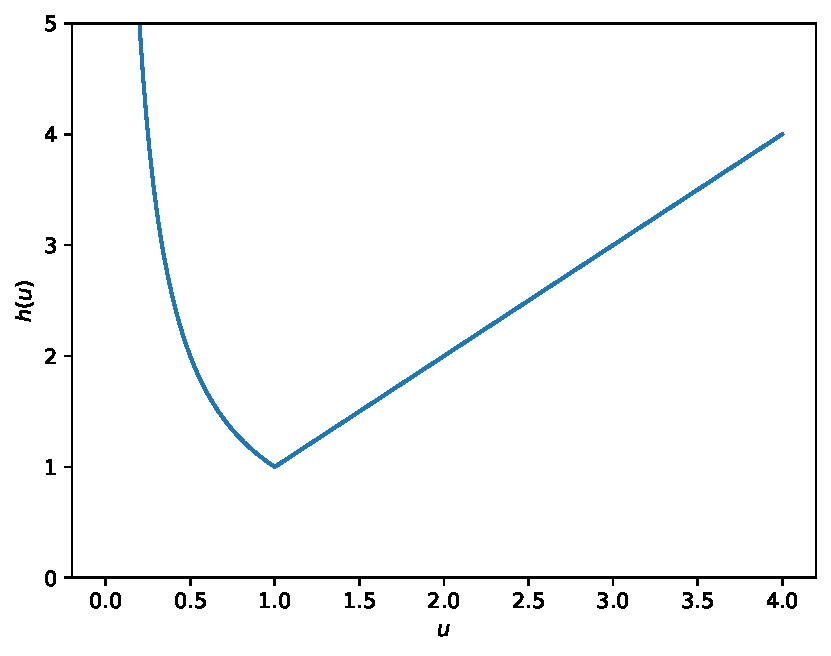
\includegraphics[width=0.55\textwidth]{figures/convex-function.pdf}
    \caption{Behaviour of the function $h(u)$.}\label{fig:convex-function}
\end{figure}

\end{document}
